\section{Cel i założenia projektowe}
    \tab Powyższy projekt oparty jest o mikrokontroler z rodziny AVR: ATmega8A.
    Komunikując się z odpowiedniki sensorami jest w stanie zlokalizować się w przestrzeni,
    oraz stworzyć prostą mapę pomieszczenia, w którym się znajduje. A następnie swobodnie poruszać się po nim.

    \subsection{Środowisko sprzętowe}
        \tab Jak wyżej wspomniano, sercem projektu jest mikrokontroler ATmega8A, a wspomnianymi modułami są odpowiednio:
        \begin{enumerate}
            \item Ultradźwiękowa czujka odległości -- HC-SR04,
            \item Trój-osiowy akcelerometr -- MMA8451,
            \item Moduł bluetooth -- HC05,
            \item Scalony mostek H -- układ L293D TexasInstruments,
            \item Silniki modelarskie z przekładniami 1:48 o napięciu znamionowym 6V,
            \item Serwo mechanizm -- SG90.
        \end{enumerate}
% 
        Zasilanie dostarczają dwa wbudowane akumulatory litowo-jonowe 18650 o napięciu znamionowym 3.7V, podniesionym za pomocą przetwornicy STEP UP (CN6009) do około 5V.
        % Zasilanie jest z dwóch akumulatorów litowo-jonowych 18650 o napięciu znamionowym 3.7V, podniesionym za pomocą przetwornicy STEP UP do około 5V.


        \subsubsection{Schemat ideowy}
            Wstawić schemat
        
    \subsection{Środowisko programowe}
        \tab Program na ATmegę został napisany w języku C/C++, z wykorzystaniem bibliotek udostępnionych przez producenta.
        Do programowania, układu zostało wykorzystane narzędzie \textit{AVRdude} wraz z programatorem \textit{USBasp}.
        Natomiast graficzny interfejs dla komputerów klasy PC, został stworzony w Pythonie, z wykorzystaniem biblioteki ,,Turtle".

    \subsection{Interfejs komunikacyjny}
        \tab Wiele nowoczesnych urządzeń wykorzystuje rozmaite standardy i interfejsy komunikacyjne do różnych celów.
        Tak samo powyższy projekt wykorzystuje kilka prostych standardów do komunikacji zarówno z użytkownikiem oraz peryferiami.

        \subsubsection{Standard UART i interfejs bluetooth}
            \tab Podstawowym sposobem komunikacji z użytkownikiem jest protokół UART, wraz z interfejsem Bluetooth.
            Standard komunikacji UART, jest to prosty dwukierunkowy asynchroniczny sposób do przesyłania danych między dwoma urządzeniami.\\
            Opis przykładowej ramki w standardzie UART:
            
            \begin{figure}[!h]
                \centering
                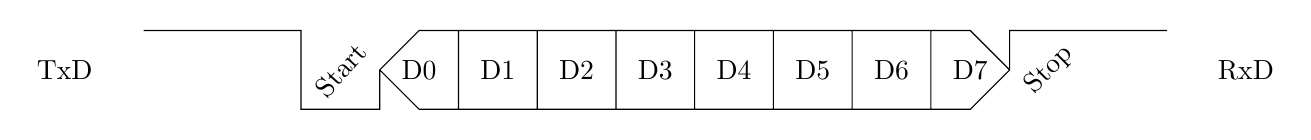
\begin{tikzpicture}
                    \draw
                    (-1, 0.5) node[]{TxD}
                    (0, 1) -- (2, 1)
                        -- (2, 0)
                        -- (3, 0)
                        -- (3, 0.5) coordinate(start) ++(-0.5, 0) node[rotate = 48]{Start}

                    (start) --++ (0.5, -0.5) -- ++ (7, 0) --++(0.5, 0.5) coordinate(stop)
                    (start) --++ (0.5, 0.5) -- ++ (7, 0) --++(0.5, -0.5)

                    (start) ++ (1, 0.5) -- ++ (0, -1) ++ (-0.5, 0.5) node[]{D0}
                    (start) ++ (2, 0.5) -- ++ (0, -1) ++ (-0.5, 0.5) node[]{D1}
                    (start) ++ (3, 0.5) -- ++ (0, -1) ++ (-0.5, 0.5) node[]{D2}
                    (start) ++ (4, 0.5) -- ++ (0, -1) ++ (-0.5, 0.5) node[]{D3}
                    (start) ++ (5, 0.5) -- ++ (0, -1) ++ (-0.5, 0.5) node[]{D4}
                    (start) ++ (6, 0.5) -- ++ (0, -1) ++ (-0.5, 0.5) node[]{D5}
                    (start) ++ (7, 0.5) -- ++ (0, -1) ++ (-0.5, 0.5) node[]{D6}
                    (start) ++ (8, 0.5) ++ (0, -1) ++ (-0.5, 0.5) node[]{D7}
                    % (start) ++ (8.5, 0) node[]{P}

                    (stop) --++(0, 0.5) -- ++(2, 0) coordinate(end)
                    (stop) ++ (0.5, 0) node[rotate = 45]{Stop}
                    (end) ++ (1, -0.5) node[]{RxD}
                        
                    ;
                \end{tikzpicture}
                \caption{Ramka danych w standardzie UART}
            \end{figure}
% 
            \noindent
            W tym projekcie komunikacja odbywa się z szybkością 9600baud'ów (Do zmiany prawie na 100\%).
            Dodatkowo, standard pozwala na przesyłanie dodatkowego bity parzystości ,,doklejanego" do końca wiadomości, jako sposób sprawdzania poprawności wysłanej wiadomości.

            Dalszą częścią kanału transmisyjnego jest przekaźnik bluetooth, który łączy się z komputerem na odpowiednim porcie szeregowym łatwym do oczytania dla programu napisanego na komputerze.

    \subsubsection{Interfejs SPI}
            % źródło: http://extronic.pl/content/60-kurs-xmega-interfejs-spi
            \tab Procesor bez programu, jest bezużytecznym kawałkiem krzemu dlatego niezwykle istotnym jest zaprogramowanie układu.
            Podstawową metodą programowania układów z rodziny ATmega jest interfejs SPI. 

            \begin{figure}[!h]
                \centering
                \begin{tikzpicture}
                    \draw
                        (0, 0) -- (0, 8) -- (1, 8) -- (1, 0) -- (0, 0)
                        (0, 1) -- (1, 1) ++ (-0.5, -0.5) node[](MD0){D0}
                        (0, 2) -- (1, 2) ++ (-0.5, -0.5) node[]{D1}
                        (0, 3) -- (1, 3) ++ (-0.5, -0.5) node[]{D2}
                        (0, 4) -- (1, 4) ++ (-0.5, -0.5) node[]{D3}
                        (0, 5) -- (1, 5) ++ (-0.5, -0.5) node[]{D4}
                        (0, 6) -- (1, 6) ++ (-0.5, -0.5) node[]{D5}
                        (0, 7) -- (1, 7) ++ (-0.5, -0.5) node[]{D6}
                                         ++       (0, 1) node[](MD7){D7}
                        (2, -1.5) -- (2, 9)

                        (8, 0) -- (8, 8) -- (9, 8) -- (9, 0) -- (8, 0)
                        (8, 1) -- (9, 1) ++ (-0.5, -0.5) node[](SD7){D7}
                        (8, 2) -- (9, 2) ++ (-0.5, -0.5) node[]{D6}
                        (8, 3) -- (9, 3) ++ (-0.5, -0.5) node[]{D5}
                        (8, 4) -- (9, 4) ++ (-0.5, -0.5) node[]{D4}
                        (8, 5) -- (9, 5) ++ (-0.5, -0.5) node[]{D3}
                        (8, 6) -- (9, 6) ++ (-0.5, -0.5) node[]{D2}
                        (8, 7) -- (9, 7) ++ (-0.5, -0.5) node[]{D1}
                                         ++       (0, 1) node[](SD0){D0}
                        (7, -1.5) -- (7, 9)

                        
                        (-2.75, -1.25) rectangle ++ (2, 1)
                        (-1.75, -0.75) node[](clk){Clk} 
                        (clk) ++ (1, 0) coordinate(clk)
                        (clk) -- ++ (0.5, 0)
                            to[short, *-] ++ (0, 1.25) coordinate(MD)
                            to[short, *-] ++ (0.25, 0)
                        (MD) -- ++ (0, 1) coordinate(MD)
                            to[short, *-] ++ (0.25, 0)
                        (MD) -- ++ (0, 1) coordinate(MD)
                            to[short, *-] ++ (0.25, 0)
                        (MD) -- ++ (0, 1) coordinate(MD)
                            to[short, *-] ++ (0.25, 0)
                        (MD) -- ++ (0, 1) coordinate(MD)
                            to[short, *-] ++ (0.25, 0)
                        (MD) -- ++ (0, 1) coordinate(MD)
                            to[short, *-] ++ (0.25, 0)
                        (MD) -- ++ (0, 1) coordinate(MD)
                            to[short, *-] ++ (0.25, 0)
                        (MD) -- ++ (0, 1) coordinate(MD)
                            to[short] ++ (0.25, 0)

                        (clk) -- ++ (10, 0) coordinate(SD)
                        (SD) to[short, -] ++ (0, 1.25) coordinate(SD)
                            -- ++(-0.25, 0)
                        (SD) to[short, *-] ++ (0, 1) coordinate(SD)
                            -- ++(-0.25, 0)
                        (SD) to[short, *-] ++ (0, 1) coordinate(SD)
                            -- ++(-0.25, 0)
                        (SD) to[short, *-] ++ (0, 1) coordinate(SD)
                            -- ++(-0.25, 0)
                        (SD) to[short, *-] ++ (0, 1) coordinate(SD)
                            -- ++(-0.25, 0)
                        (SD) to[short, *-] ++ (0, 1) coordinate(SD)
                            -- ++(-0.25, 0)
                        (SD) to[short, *-] ++ (0, 1) coordinate(SD)
                            -- ++(-0.25, 0)
                        (SD) to[short, *-] ++ (0, 1) coordinate(SD)
                            -- ++(-0.25, 0)

                        (MD7) ++ (0.5, 0) coordinate (MD7)
                        (SD0) ++ (-0.5,0) coordinate (SD0)
                        (MD0) ++ (0.5, 0) coordinate (MD0)
                        (SD7) ++ (-0.5,0) coordinate (SD7)

                        (MD7) -- (SD0)
                        (MD0) -- (SD7)
                        
                        (MD7) ++ (4, 0) -- ++ (-0.2, 0.2)
                        (MD7) ++ (4, 0) -- ++ (-0.2, -0.2)
                        (MD7) ++ (2.2, 0) node[above]{MOSI}
                        (SD7) ++ (-2.2, 0) node[above]{MOSI}

                        (MD0) ++ (4, 0) -- ++ (0.2, 0.2)
                        (MD0) ++ (4, 0) -- ++ (0.2, -0.2)
                        (MD0) ++ (2.2, 0) node[above]{MISO}
                        (SD0) ++ (-2.2, 0) node[above]{MIS0}

                        (MD7) ++ (0, 1) node[]{MASTER}
                        (SD0) ++ (0, 1) node[]{SLAVE}
                    ;

                \end{tikzpicture}
                \caption{Schemat interfejsu SPI}
            \end{figure}
            \noindent
            W przeciwieństwie do poprzednio omawianego interfejsu,
            SPI jest interfejsem typu Master-Slave -- wyróżniamy układ sterujący (Master),
            którego zadaniem jest wyznaczenie taktowania zegara 
            oraz zarządzanie magistralą układami układami podrzędnymi (Slave), poprzez wystawienie stanu aktywnego na pinie \textit{,,CS"}.

            % Dodatkowo, urządzenia slave posiadają specjalne wejście ,,CS", których aktywacja zezwala na komunikację za pomocą protokołu SPI.
        

        \subsubsection{Interfejs Two Wire}
            